\documentclass[rep.tex]{subfiles}
\begin{document}

\chapter{Zadanie 6}
\label{zad6}
\section{Treść}
Zaprojektować niesymetryczną linię paskową, rys~\ref{fig:zad6:microstrip}, o impedancji charakterystycznej~$Z_0 = 50~\Omega$.
Podłoże linii stanowi dielektryk o~$\epsilon_r = 2.56$, $\mu_r = 1$ i grubości~$h =  1.4~mm$.
Obliczenia wykonać, przy założeniu, że grubość przewodu wewnętrznego~$t =  0.0035~mm$.
Obliczyć długość fali w tak zaprojektowanej linii wiedząc, ze jej częstotliwość~$f = 1.5~GHz$.

\begin{figure}[!htbp]
  \centering
  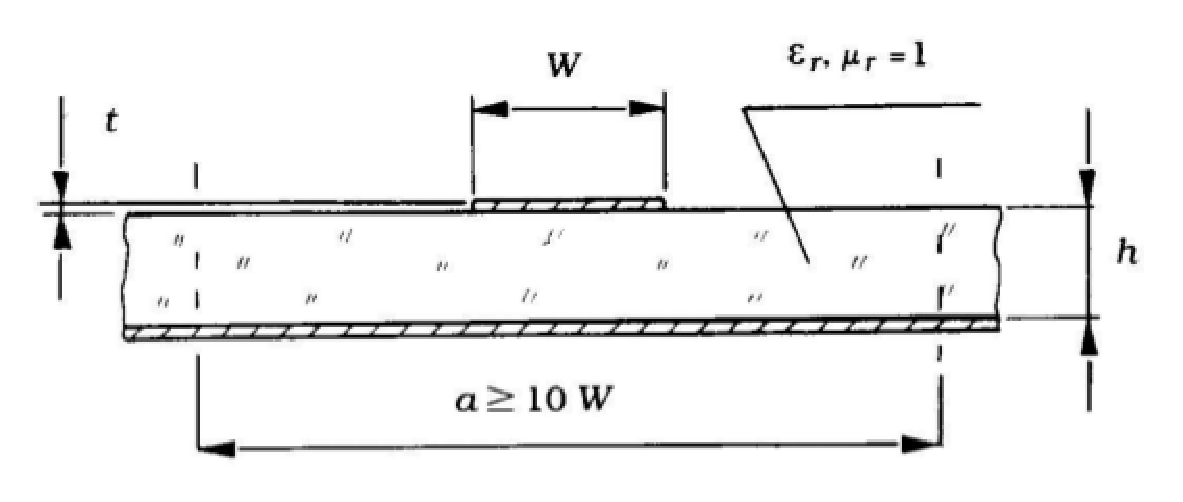
\includegraphics[scale=0.5]{fig/zad6/microstrip}
  \caption{Nieymetryczna linia paskowa}
  \label{fig:zad6:microstrip}
\end{figure}

\section{Rozwiązanie}
\subsection{Szerokość linii}
Niesymetryczna linia paskowa, ze względu na niezwykle łatwe i tanie wytwarzanie, jest jedną z najpopularniejszych prowadnic falowych.
Pomimo swojej popularności ciągle nie są znane analityczne zależności projektowe.
Dlatego na potrzeby projektu posłużono się wzorami zawartymi w~\cite{obwody}.

Rozwiązanie zadania polega na znalezieniu szerokości paska, jaki będzie tworzył linie o wymaganej impedancji.
W tym celu należy numerycznie rozwiązanć równanie:
\begin{equation}
  Z_0(u, f) - Z_0 = 0 \label{eqn:zad6:target}
\end{equation}
gdzie:\\
\begin{tabular}{l @{ - } l}
  $Z_0$ & wymagana impedancja \\
  $u = \frac{W}{h}$ & stosunek od którego zależy impedancja \\
  $f$ & częstotliwość pracy
\end{tabular}

Impedancje linii oblicza się wzorem:
\begin{equation}
  Z_0(u, f) = \frac{60}{\sqrt{\epsilon_{ef}(f)}} \ln\Bigg[\frac{f(u)}{u} + \sqrt{1 + \bigg(\frac{2}{u}\bigg)^2}\Bigg] \label{eqn:zad6:Z0}
\end{equation}
Pomocnicze równania niezbędne do obliczenia impedancji zawartę są~w~\cite{obwody}.

Należy zwrócić uwagę na to, że wzór~\ref{eqn:zad6:Z0} jest słuszny w przypadku gdy przewód wewnętrzny jest nieskończenie cienki~$t = 0$.
Gdy chcemy uwzględnić grubość paska należy od~$u$ dla którego równanie~\ref{eqn:zad6:target} jest spełnione odjąć poprawkę:
\begin{equation}
  \Delta u = \frac{t}{2 \pi h}\ln\Big( 1 + \frac{4eh}{t\operatorname{cth}^2\sqrt{6.517u}}\Big)\Big(1 + \frac{1}{\operatorname{ch}\sqrt{\epsilon_r - 1}}\Big) \label{eqn:zad6:du}
\end{equation}

Uwzględniając to wszystko zadanie rozwiązano korzystając z algorytmu Newtona-Raphsona napisanego dla poprzednich zadań.
Wartość szerokości paska~$w$ dla którego impedancja wynosi~$50~\Omega$ wynosi~$w = 3.90022750273~mm$.

\subsection{Długość fali}
Pole elektromagnetyczne w niesymetrycznej linii paskowej rozchodzi się, częściowo poprzez dielektryk a częściowo w powietrzu.
Dlatego należy obliczyć efektywną prznikalność dielektryczną:
\begin{align}
  \epsilon_{eff}(u, f) &= \frac{\epsilon_{eff}(u, 0) + \epsilon_rp(u, f)}{1 + p(u, f)}
  \epsilon_{eff}(u, 0) &= \frac{\epsilon_r + 1}{2} + \frac{\epsilon_r - 1}{2}\Big(1 + \frac{10}{u}\Big)^{-a(u)\times b(\epsilon_r)}
\end{align}

Mając obliczoną efektywną prznikalność elektryczną można obliczyć długość fali rozchodzącej się w linii.
\begin{equation}
  \lambda = \frac{c_{osr}}{f} = \frac{c}{\sqrt{\epsilon_{eff}}\times f} \label{eqn:zad6:lambda}
\end{equation}

Dla wartości określonych w treści zadania długość fali rozchodzącej się w zaprojektowanej linii wynosi:~$\lambda = 13.6746810073~cm$.
\end{document}
